\documentclass[UTF8]{ctexart}
\usepackage{xcolor}
\usepackage{graphicx}
\usepackage{geometry}
\usepackage{section}
\usepackage{subfigure}
\usepackage{float}
\usepackage{listings}
\geometry{top=3.0cm, bottom=1.0cm, right=1.5cm, left=1.5cm}

%\lstset{basicstyle=\sffamily, keywordstyle=\bfseries,commentstyle=\rmfamily\itshape,stringstyle=\ttfamily }
\lstset{numbers=left,
	numberstyle=\tiny,
	basicstyle=\sffamily, 
	keywordstyle=\bfseries,
	commentstyle=\rmfamily\itshape,
	stringstyle=\ttfamily
	keywordstyle=\color{blue!70}, commentstyle=\color{red!50!green!50!blue!50},
	frame=shadowbox,
	rulesepcolor=\color{red!20!green!20!blue!20}
}



\title{\huge{实验三:滤波器设计和滤波器的特性分析}}
\author{\textbf{PB18020520 \qquad 刘洪健}}
\date{\today}

\begin{document}
\maketitle
\tableofcontents
\section{实验目的}
\begin{enumerate}
	\item 掌握matlab中滤波器设计工具fdatool的方法
	\item 掌握IIR滤波器设计的方法
	\item 掌握FIR滤波器设计的方法
	\item 了解IIR 和 FIR 滤波器的特性
	\item 掌握滤波器性能分析的方法
	\item 掌握sptool工具的使用
\end{enumerate}
\section{实验内容}
\subsection{IIR滤波器}
\subsubsection{高通滤波器}
\hspace*{2em}利用Chebyshev模型设计,按照要求:$f_p=0.3Hz \quad {\alpha}_p=0.8dB \quad f_s=0.2Hz \quad {\alpha}_s=20dB$

利用matlab的cheby函数等设计,\textbf{代码如下}
\begin{lstlisting}[language=matlab]
	Fs = 1;  % Sampling Frequency

	fs = 0.2*2;         % Stopband 
	fp = 0.3*2;         % Passband 
	As = 20;          % Stopband Attenuation (dB)
	Ap = 0.8;         % Passband Ripple (dB)
	[n, Wn] = cheb1ord(fp, fs, Ap, As);
	[b, a] = cheby1(n, Ap, Wn, 'high');
	fvtool(b,a);
\end{lstlisting}
得到的H(Z)系数为

b:  0.0262   -0.1047    0.1570   -0.1047    0.0262 \\
\hspace*{2em}a:  1.0000    1.5289    1.6537    0.9452    0.2796\\
\[
H(Z)=\frac{0.0262-0.1047Z^{-1}+0.157Z^{-2}-0.1047Z^{-3}+0.0262Z^{-4}}{1+1.5289Z^{-1}+1.6537Z^{-2}+0.9452Z^{-3}+0.2796Z^{-4}}
\]
利用fvtool工具查看其幅频特性曲线,如下图
\begin{figure}[H]
	\centering
	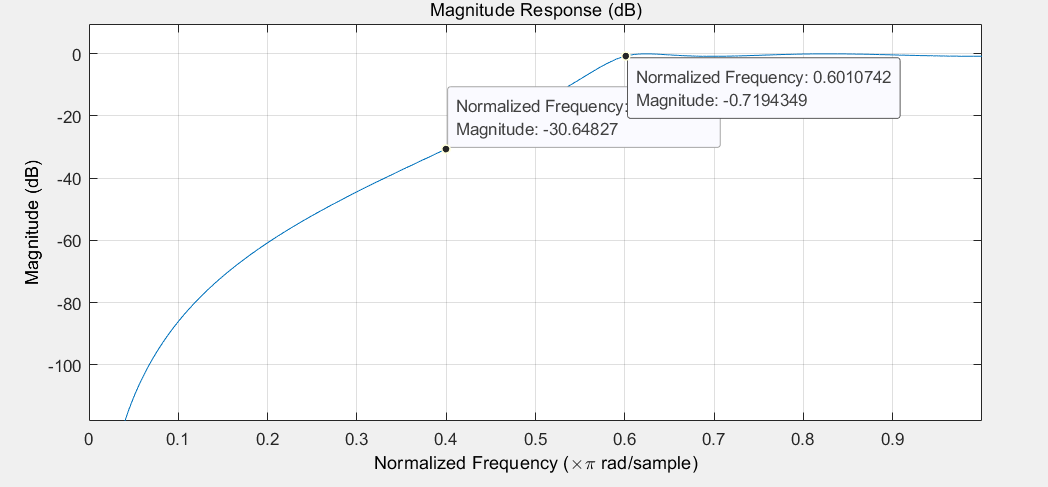
\includegraphics[scale=0.8]{figs/iir1}
	\caption{IIR高通滤波器}
\end{figure}
可以看出,在通带和阻带的起伏均满足要求。同时,根据幅频特性曲线,在通带内并不是严格下降的,而是有一定波纹的,也符合chebyshev模型的特点,同时滤波器只用了5阶就实现了要求。
\subsubsection{低通滤波器}
设计数字低通滤波器,其中的性能要求是::$f_p=0.2Hz \quad {\alpha}_p=1dB \quad f_s=0.3Hz \quad {\alpha}_s=25dB$\\
我采用Butterworth法设计,\textbf{代码如下}
\begin{lstlisting}[language=matlab]
	Fs = 1;  % Sampling Frequency
	
	fs = 0.3*2;         % Stopband 
	fp = 0.2*2;         % Passband 
	As = 25;          % Stopband Attenuation (dB)
	Ap = 1;         % Passband Ripple (dB)
	[n, Wn] = buttord(fp, fs, Ap, As);
	[b, a] = butter(n, Wn);
	fvtool(b,a);
\end{lstlisting}
得到的H(Z)系数为\\
\hspace*{2em}b:  0.0179    0.1072    0.2681    0.3575    0.2681    0.1072    0.0179 \\
\hspace*{2em}a:  1.0000   -0.6019    0.9130   -0.2989    0.1501   -0.0208    0.0025 \\
\[
H(Z)=\frac{0.0179+0.1072Z^{-1}+0.2681Z^{-2}+0.3575Z^{-3}+0.2681Z^{-4}+0.1072Z^{-5}+0.0179Z^{-6}}{1-0.6019Z^{-1}+0.913Z^{-2}-0.2989Z^{-3}+0.1501Z^{-4}-0.0208Z^{-5}+0.0025Z^{-6}}
\]
利用fvtool查看其幅频特性曲线,如下图
\begin{figure}[H]
	\centering
	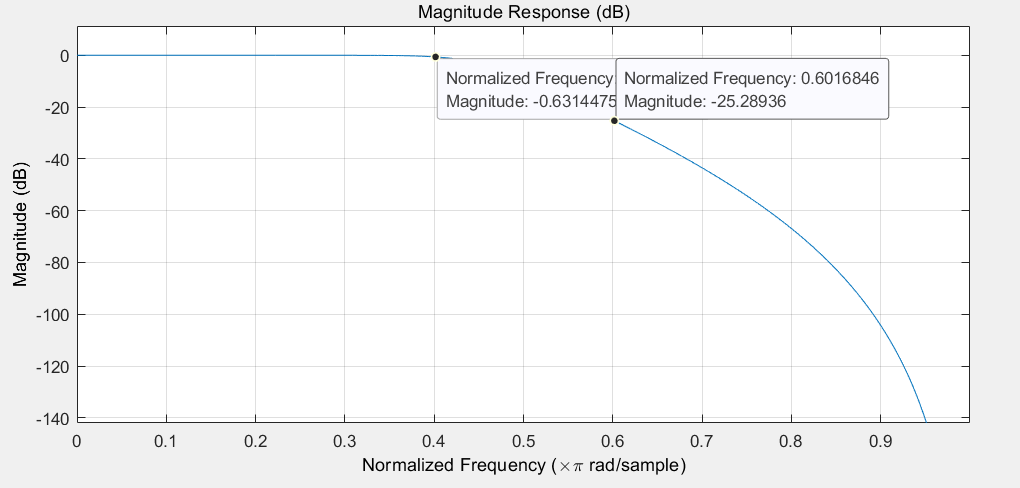
\includegraphics[scale=0.8]{figs/iir2}
	\caption{IIR低通滤波器}
\end{figure}
可以看出,在通带和阻带的起伏均满足要求。同时,根据幅频特性曲线,幅频曲线严格下降,符合Butterworth模型。
\subsubsection{Butterworth带通滤波器}

 
	
\end{document}